% This is part of Un soupçon de physique, sans être agressif pour autant
% Copyright (C) 2006-2009,2016
%   Laurent Claessens
% See the file fdl-1.3.txt for copying conditions.

\section{Miroirs sphériques}
%---------------------------

Cette section va parler de \href{http://fr.wikipedia.org/wiki/Miroir_sphérique}{miroirs sphériques}. Ce sont des calottes sphériques. Selon que la surface intérieure ou extérieure est réfléchissante, le miroir est dit \defe{concave}{} ou \defe{convexe}{}.

L'optique des miroirs sphériques se résume en trois règles simples.
\setcounter{numloiphyz}{0}		% Note qu'il faudra souvent le remettre à zéro ce compteur. Genre à tous les coups.
\begin{loiphyz}\label{PgLoiMirSph}
Tout rayon passant réellement ou virtuellement par le centre de courbure se réfléchit sur lui-même.
\end{loiphyz}

\begin{loiphyz}
Tout rayon parallèle à l'axe principal se réfléchit en passant réellement ou virtuellement par un point appelé \defe{foyer}{}.
\end{loiphyz}

\begin{loiphyz}
Tout rayon passant réellement ou virtuellement par le foyer se réfléchit parallèlement à l'axe principal.
\end{loiphyz}
Le foyer dont il est question dans la seconde loi se trouve sur l'axe principal juste au milieu entre le centre et le miroir. La distance entre le miroir et le foyer $F$ (voir la figure \ref{FigPasageFoyer}) s'appelle la \defe{distance focale}{} et se note $f$ :
\begin{equation}
  f=\frac{ R }{ 2 }
\end{equation}
où $R$ est le rayon du miroir. La figure \ref{FigPasageFoyer} montre des rayons lumineux qui sont réfléchis vers le foyer.


\begin{figure}
\centering
\subfigure[Passage réel, miroir concave]{%
    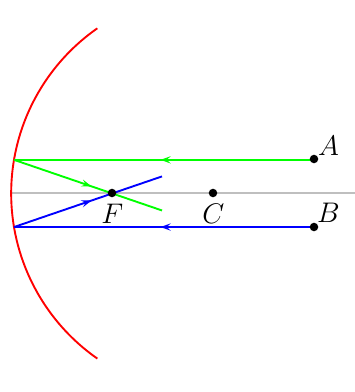
\includegraphics{fig12694_1.png}
}
\subfigure[Passage virtuel, miroir convexe]{%
    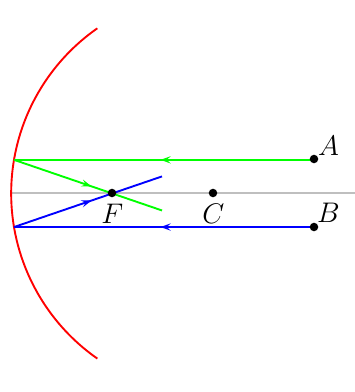
\includegraphics{fig12694_1.png}
}
\caption{Miroir sphérique : admirez comme tous les rayons parallèles à l'axe se réfléchissent en passant par le foyer !}  \label{FigPasageFoyer}
\end{figure}

\subsection{Construction de l'image d'un objet}
%----------------------------------------------

Muni des lois de la page \pageref{PgLoiMirSph}, nous sommes à même de construire l'image d'un objet $AB$. La figure \ref{FigMiroirSpherique} donne un exemple de la construction de l'image d'un point. Lorsqu'on a un segment $AB$ dont il faut calculer l'image, le plus simple est de choisir l'axe optique de telle façon à contenir le point $A$ et être perpendiculaire à $AB$. 

\begin{figure}
\centering
    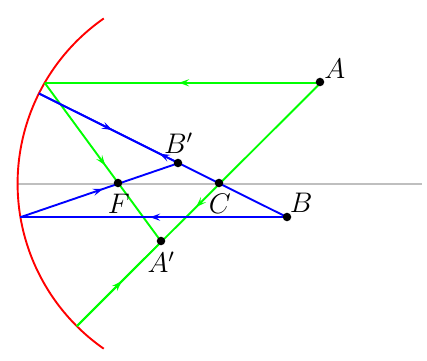
\includegraphics{fig29073_1.png}
\caption{Miroir sphérique : deux exemples de construction d'images de points. Un peu confus hein ? Essaie de refaire le dessin toi-même, et ça te paraîtra plus simple.}  \label{FigMiroirSpherique}
\end{figure}

Regardons pas à pas la construction de la figure \ref{FigConcUn}. Sur la figure \ref{FigConcUnPara}, nous avons tracé le rayon issu de $B$, et trouvé son intersection avec le miroir. En vertu d'une des lois (laquelle ?) de la page \ref{PgLoiMirSph}, ce rayon va se refléter en passant par le foyer (qui se trouve, rappelons-le, au milieu du segment d'axe optique joignant le centre du miroir et le miroir), comme montré sur la figure \ref{FigConcUnFoyer}. Pour terminer de fixer l'objet, on construit l'autre chemin facile : celui du rayon issu de $B$ qui tombe sur le miroir en passant par le centre. Celui-là est dessiné sur la figure \ref{FigConcUnCentre}.

\begin{figure}
\centering
\subfigure[D'abord, tracer le rayon issu de $A$ parallèlement à l'axe optique, et trouver le point $I$ où ce rayon tombe sur le miroir]{%
    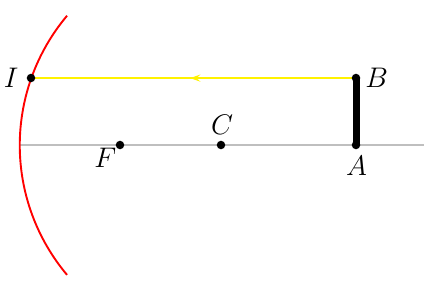
\includegraphics{fig7954_1.png}
\label{FigConcUnPara}
}
\subfigure[Ce rayon se reflète en passant par le foyer]{%
    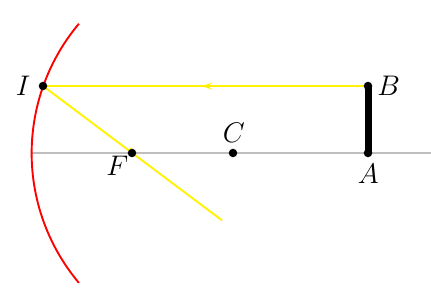
\includegraphics{fig7954_2.png}
\label{FigConcUnFoyer}
}
\subfigure[Le rayon issu de $B$ passant par le centre optique est reflété sur lui-même.]{%
    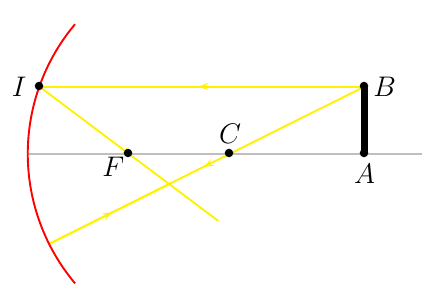
\includegraphics{fig7954_3.png}
\label{FigConcUnCentre}
}
\subfigure[L'intersection des deux rayons donne l'image de $B$, et permet de construire l'image de l'objet]{%
    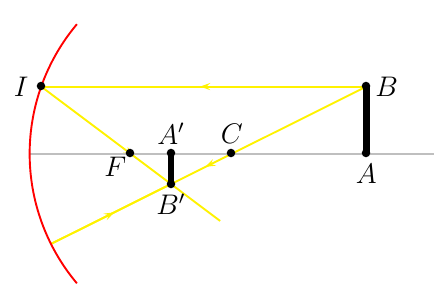
\includegraphics{fig7954_4.png}
\label{FigConcUnReponse}
}
\caption{Construction de l'image d'un objet}  \label{FigConcUn}
\end{figure}

Admirons maintenant sur la figure \ref{FigCasConcaves} différents cas que l'on peut trouver parmi les miroirs concaves. 

Il faut en particulier remarquer le passage virtuel sur la figure \ref{FigCasConcavesa} : le trajet que les rayons font en réalité est de se refléter sur le miroir et de diverger (contrairement aux deux autre cas).

\begin{figure}
\centering
\subfigure[Si l'objet se trouve au-delà du centre de courbure, l'image est renversée et plus petite que l'objet. De plus l'image est faire de rayons issus de l'objet lui-même, elle est donc réelle.]{
    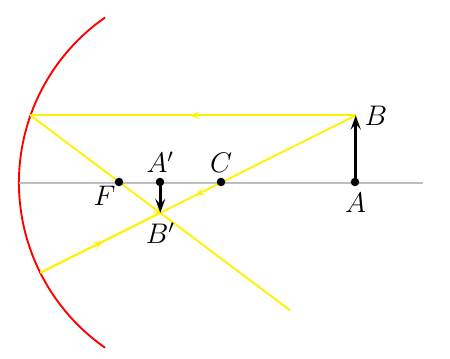
\includegraphics{fig28708_1.png}
\label{SubFigAudela}
}
\subfigure[Si l'objet se trouve entre le centre de courbure et le foyer, l'image est renversée, plus grande que l'objet et réelle.]{
    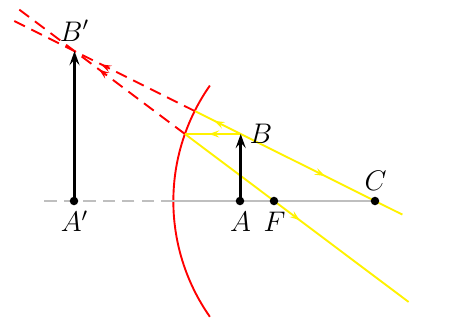
\includegraphics{fig28708_3.png}
}
\subfigure[Si l'objet se trouve entre le foyer et le miroir, l'image est droite, plus grande que l'objet et virtuelle. Les lignes en traits discontinus ne correspondent pas à un trajet que la lumière suit réellement : il n'y a pas de lumière à cet endroit.]{
    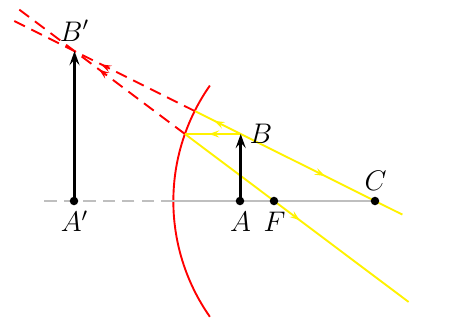
\includegraphics{fig28708_3.png}
\label{FigCasConcavesa}
}
\caption{Différents cas possibles avec un miroir concave.}  \label{FigCasConcaves}
\end{figure}

Le cas des miroirs convexes est exactement le même, sauf qu'on a plus souvent des passages virtuels. En suivant la méthode montrée à la figure \ref{FigConcUn}, nous obtenons la figure \ref{FigConvexeEx}.

\subsection{Quelque formules}
%----------------------------

En étudiant des triangles semblables sur la figure \ref{SubFigAudela} par exemple, nous pouvons établir les formules suivantes :
\begin{subequations}
\begin{equation}
  \frac{1}{ d }+\frac{1}{ d' }=\frac{1}{ f }\\
\end{equation}
\begin{equation}
   -\frac{ h' }{ h }=\frac{ d' }{ d }
\end{equation}
\end{subequations}
où $d'=\| SA' \|$ est la distance entre le miroir et l'image de l'objet, $d=\| SA \|$ est celle entre le miroir et l'objet, $h=\| AB \|$  et $h'=\| A'B' \|$ sont les tailles respectivement de l'objet et de son image ($f$ est la distance focale, c'est à dire la moitié du rayon du miroir sphérique). Nous prenons les conventions suivantes :
\begin{align*}
   f&=\text{ distance focale}\\
	&\quad >0\text{ pour un miroir concave}\\
	&\quad <0\text{ pour un miroir convexe}\\
  d&=\text{ distance de l'objet au miroir,}\\
  d'&=\text{ distance de l'image au mioir}\\
	&\quad >0\text{ pour une image réelle}\\
	&\quad <0\text{ pour une image virtuelle}\\
  h&=\text{ hauteur de l'objet}\\
  h'&=\text{ hauteur de l'image}\\
	&\quad >0\text{ pour une image droite}\\
	&\quad <0\text{ pour une image renversée}\\
\end{align*}
Le rapport $h'/h$ est souvent appelé l'\defe{agrandissement}{} du miroir.

\begin{figure}
\centering
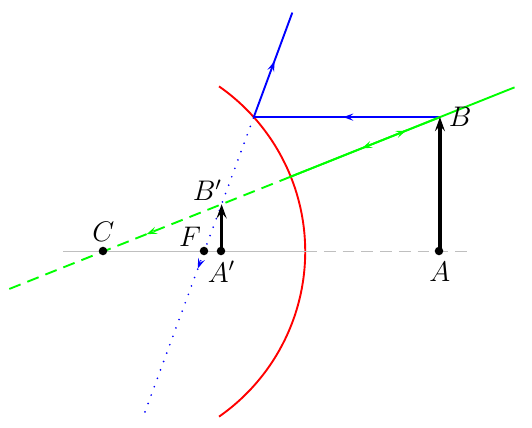
\includegraphics{fig27144_1.png}
\caption{L'image est droite, plus petite que l'objet et virtuelle.}  \label{FigConvexeEx}
\end{figure}
